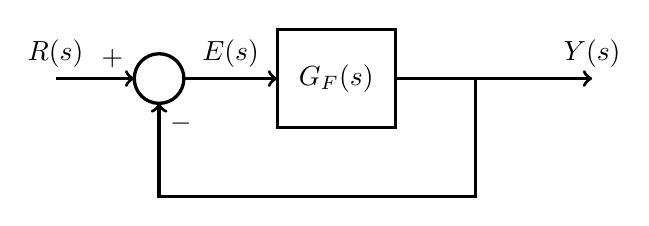
\begin{tikzpicture}[inner sep=0pt,outer sep=0pt,very thick,
sysblock/.style={draw,rectangle,inner sep=2pt,minimum width=1.5cm,minimum height=1.25cm,very thick}]

\draw (0,0) node[draw,circle] (sum) {$\rule{0pt}{18pt}$};
\draw (2.25,0) node[sysblock] (a) {$G_F(s)$};
\draw (4,0) node (c) {};

\draw[<-] (sum.180) node[above left=4pt] {$+$} -- ++(-1,0) node[above=4pt] {$R(s)$};
\draw[->] (sum.0) -- node[pos=.5,above=4pt] {$E(s)$} (a.180);
\draw[->] (a.0) -- ++(2.5,0) node[above=4pt] {$Y(s)$};
\draw[->] (c.0) -- ++(0,-1.5) -| (sum.-90) node[below right=4pt] {$-$};

\end{tikzpicture}